\documentclass[11pt]{article}
\usepackage{times}
\usepackage{graphicx}
\usepackage[top=1.0in,bottom=1.0in,left=0.5in,right=0.5in]{geometry}
\usepackage[super]{natbib}
\usepackage{url}

\begin{document}
\bibliographystyle{plain}%Choose a bibliograhpic style
\title{\textbf{A CS296 Project Report by Group 03.}}
\date{\today}
\author{Anurag Shirolkar \\ (120050003) \\ anuragshirolkar@cse.iitb.ac.in
        \and Deepanjan Kundu \\ (120050009) \\ deepanjan@cse.iitb.ac.in
        \and Syamantak Naskar \\ (120050016) \\ syamantaknaskar@cse.iitb.ac.in}
\maketitle
\clearpage
\tableofcontents
\clearpage
\section{INTRODUCTION}
\subsection{Aim}
This is the design of a steam engine. A steam engine is a heat engine that performs mechanical work using steam as its working fluid. Gas particles are treated as small spheres in this simulation.

\subsection{Comparison between Original and Implemented Design}
\begin{center}
  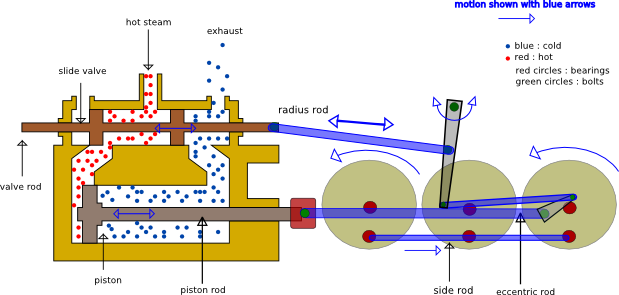
\includegraphics[width=\textwidth,height=\textheight,keepaspectratio]{loco.png}
  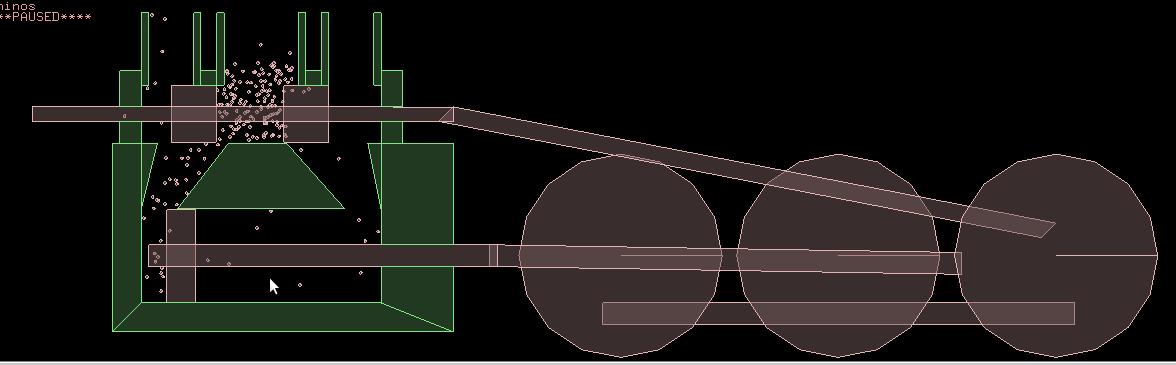
\includegraphics[width=\textwidth,height=\textheight,keepaspectratio]{working.png}
  Original Design and The Implemented Design
\end{center}
As we can see from the figures above, the two designs are pretty much the same. We have removed some of the unnecessary parts of the design e.g. the joints between different objects, the vertical rod pivoted at the upper end (called as expansion link). As well as we've made some necessary changes in the shapes and sizes of some objects like piston for better calibration.

\subsection{Working}
The model is based on the pressure difference created by hot and (relatively) cold steam on either side of the piston. The steam engine works in two steps as follows\cite{wiki}:
\begin{itemize}
\item \textbf{Valve rod in position 1: } The hot steam enters through the intake port and move the piston to the right. The movement of the piston in turn removes the cold steam out of the chamber through exhaust port. The movement of the piston also rotates the wheel which then changes the position of the valve rod from position 1 to position 2.
\item \textbf{Valve rod in position 2: } all the movements of the valve rod, piston and the particles is symmetrical to the first step. This completes one rotation of the wheel.
\end{itemize}
The other two wheels are connected to the third wheel through side rod so they rotate along with the third wheel.\\
Because of the friction between various parts of the engine and the vibrating motion of the piston and valve rod the engine settles at a certain equilibrium speed.

\section{TIMING}
The conclusions have been made using first three graphs which covers variation of all kinds of time variables with iteration value.
The graphs have been generated by using a graph generated for iteration value=1500 and 10 reruns.
\subsection{Loop Time}
\begin{center}
  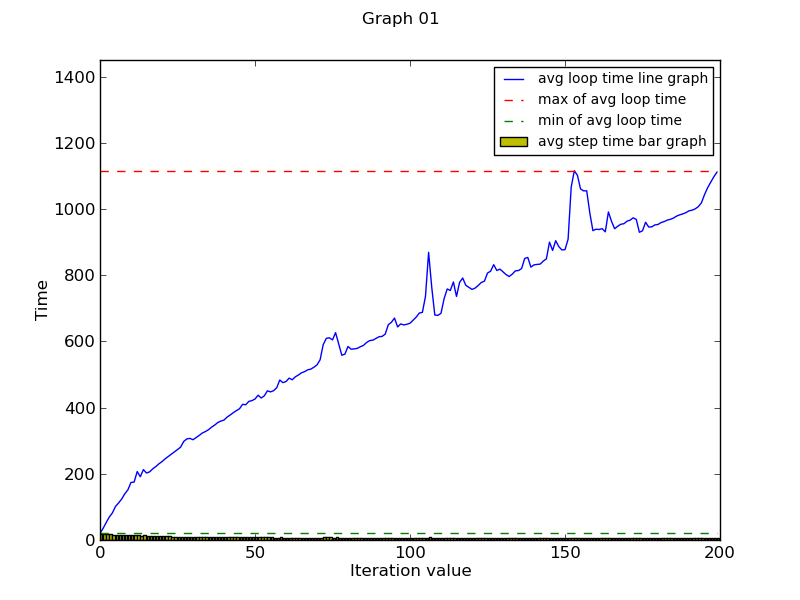
\includegraphics[scale=.5]{g03_plot01.png}
\end{center}
The loop time describes the time taken by the for loop to run. From the above graph one can conclude that it varies linearly with the iteration value as expected from the system.The for loop time which has been considered is the total for loop time over all the iterations and hence is larger than even the step time.The graph 1 clearly shows that step time graph lies very close to the zero value.
\subsection{Collision, Velocity and  Other Timings} 
\begin{center}
  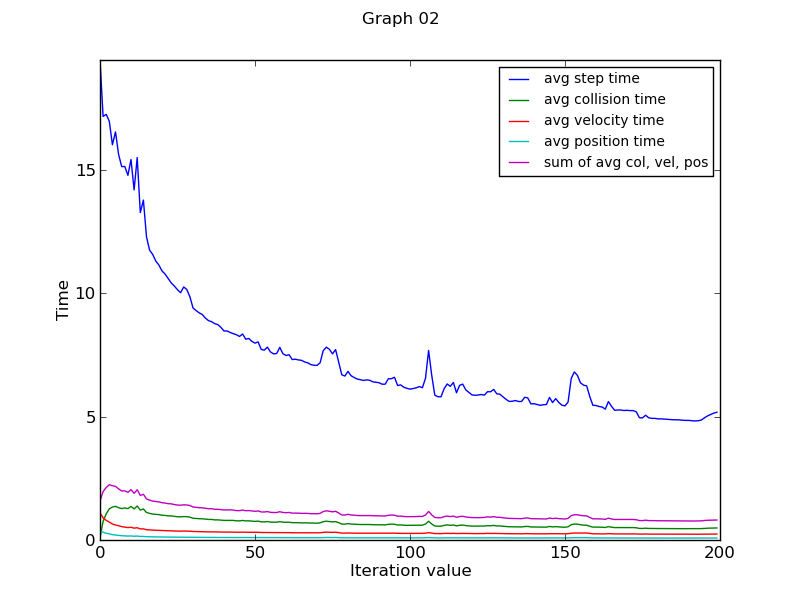
\includegraphics[scale=0.75]{g03_plot02.png}
\end{center}
The observations and inferences made are :
\begin{itemize}
\item Step time is largest among the collision,velocity ,position times.The order is Step time is greater than sum of the average collision,velocity and position time is greater than average velocity time.However the average collision and position time are very close to each other.
\item There is a variation in the nature of graph as well.For small iteration values all the different types of times decrease and the n reaching a minimum rises and then becomes fairly constant.
\item The inference that could have been drawn is that initially the number of moving objects are close to zero and we need to fix all the different parameters.However later we could recursively find the values and the number of moving objectsis the same,hence decreasing the time.However the no. of moving objects increase later(like falling of dominoes and balls)  and hence we see a slight increase in the graph which later becomes constant as the parameters are easily found and moving objects are also constant. 
\end{itemize}
\subsection{Variation in Time over Reruns}
\begin{center}
  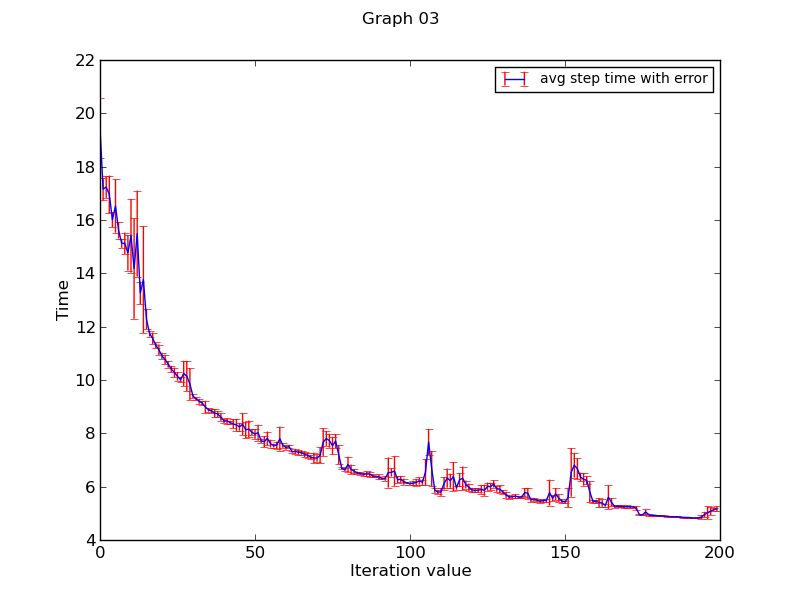
\includegraphics[scale=.75]{g03_plot03.png}
\end{center}
The error bars in graph clearly show that there is variation in running time in different reruns.This is primarily due to the different  processes running through out the system.
\subsection{Effects of Memory Heavy and CPU Heavy Processes}
This time largely depends on the nuber of cores in the system .The observation have been made on the basis of the NSL systems.
Effect of memory and cpu extensive processes(Games and libre office and several other programs and cpying and downloading processes.)
We expected that the system would slow down.However CPU processes didnot affect the timings as much the memory heavy processes .For small iteration values the change is almost nothing but the difference is a little evident at high values like 1500.The differences are not visible in graph as differences are of few milliseconds for the total loop time.\\
This happened because we were not able  to reach complete cpu usage.
However the point to note is that given complete Cpu usage the program will take a lot of time for running(about 40 percent).How ever if we are not able to push to those limits then only memory processes have some effect. 
\subsection{Difference between Time and Get Time Of Day}
\begin{center}
Number of iterations: 10000\\
Average time per step is 2.1495 ms\\
Average time for collision is 0.1606 ms\\
Average time for velocity updates is 0.1327 ms\\
Average time for position updates is 0.0606 ms\\
Total loop time is 25063.6270 ms\\
real	0m25.073s\\
user	0m25.085s\\
sys	0m0.000s\\
\end{center}
Time has three types:real,user and system.Time we need to see is user time.This time covers(time for user code processes) the entire time from the start of the program to the end  and  gettimeofday  just calculates the difference between the starting and end times of the for loop.Hence the time taken by the time command is greater than get time of day. 
\section{PROFILING}
The profile shows which function is called from where and what percentage of the time it uses.
This part covers both type of profiling using debug and release type of builds.
Perf has been used to generate the profiles.The profile info is stored in the form of .dat files.
\subsection{Debug vs Release}
Debug and release are both different types of builds,hence we use different cmake commands for both of them.Also release has a lesser running time than debug.This happens because  of the -On option which helps in internal optimizing.What it does is inline function calls and hence reduces the time.How ever the compilation time  of debug  is less than release.There is also significant difference 
Release Profile has lesser number of calls as compared to  Debug profile in the graph because of optimization.
\subsection{Debug Profiling Report}
Debug profile report has about 2Kcycles for 100 iterations.The maximum time was taken by b2World.This covers about 13\% of the time.The operator like +,*,- and functions like b2World, b2Contactmanager and b2 Vec2 consume 
a significant time.
\begin{center}
  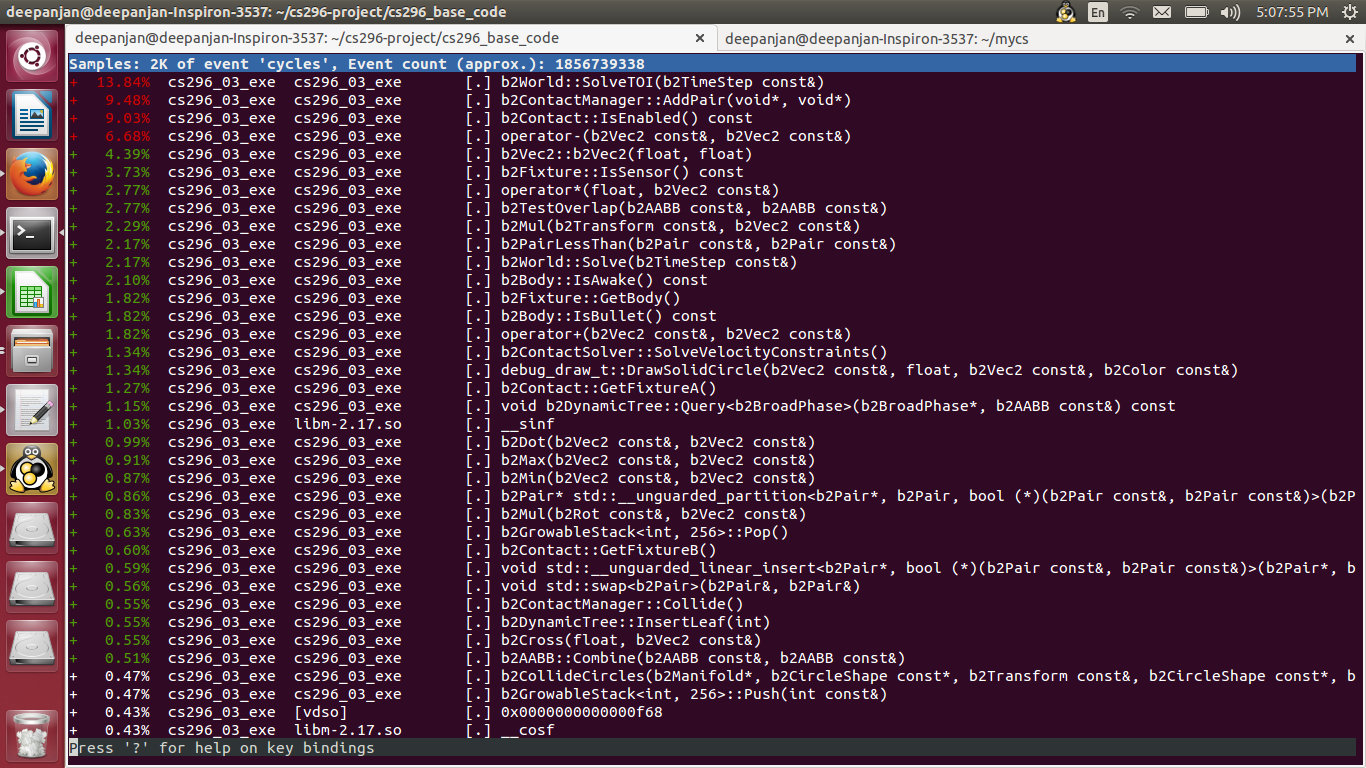
\includegraphics[scale=.25]{debug.png}
\end{center}
\subsection{Release Profiling Report}
Release profile report shows 1K cycles for 10000 iterations. The maximum overhead is taken for the symbol b2World.It uses a shared library and occupies 30\% of the time.
The operators like +,* consume a lot of time and functions like b2 ContactManager consumes 20\% of the time, b2World:collide and operators consumes alot of time.
\begin{center}
  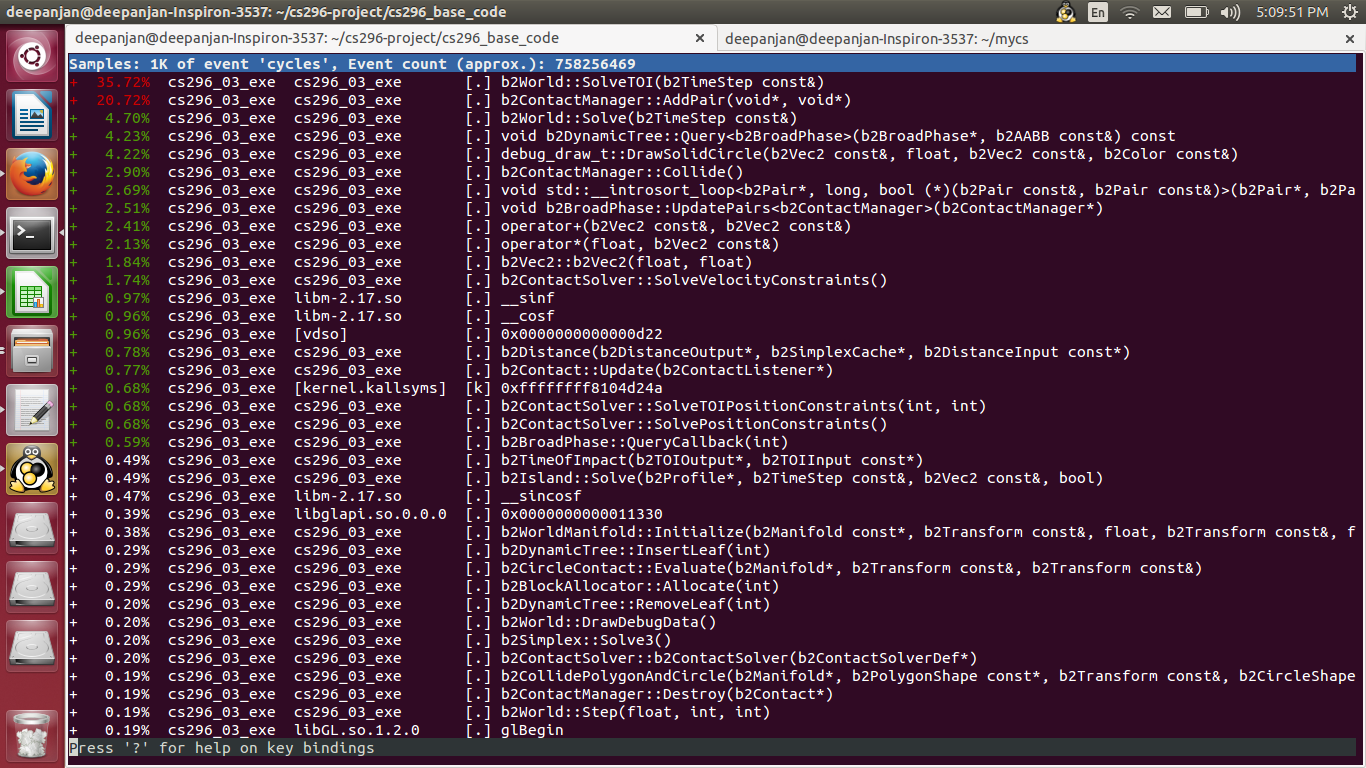
\includegraphics[scale=.3]{release.png}
\end{center}
\subsection{Callgraphs}
Call graph,a graph showing the callee-caller relationship between functions, annotated with different information on the edges has also been generated from a python script.\\
The graph has arrows representing percentages and color represents how much \% of time that function uses.

\subsubsection{Debug}
\begin{center}
  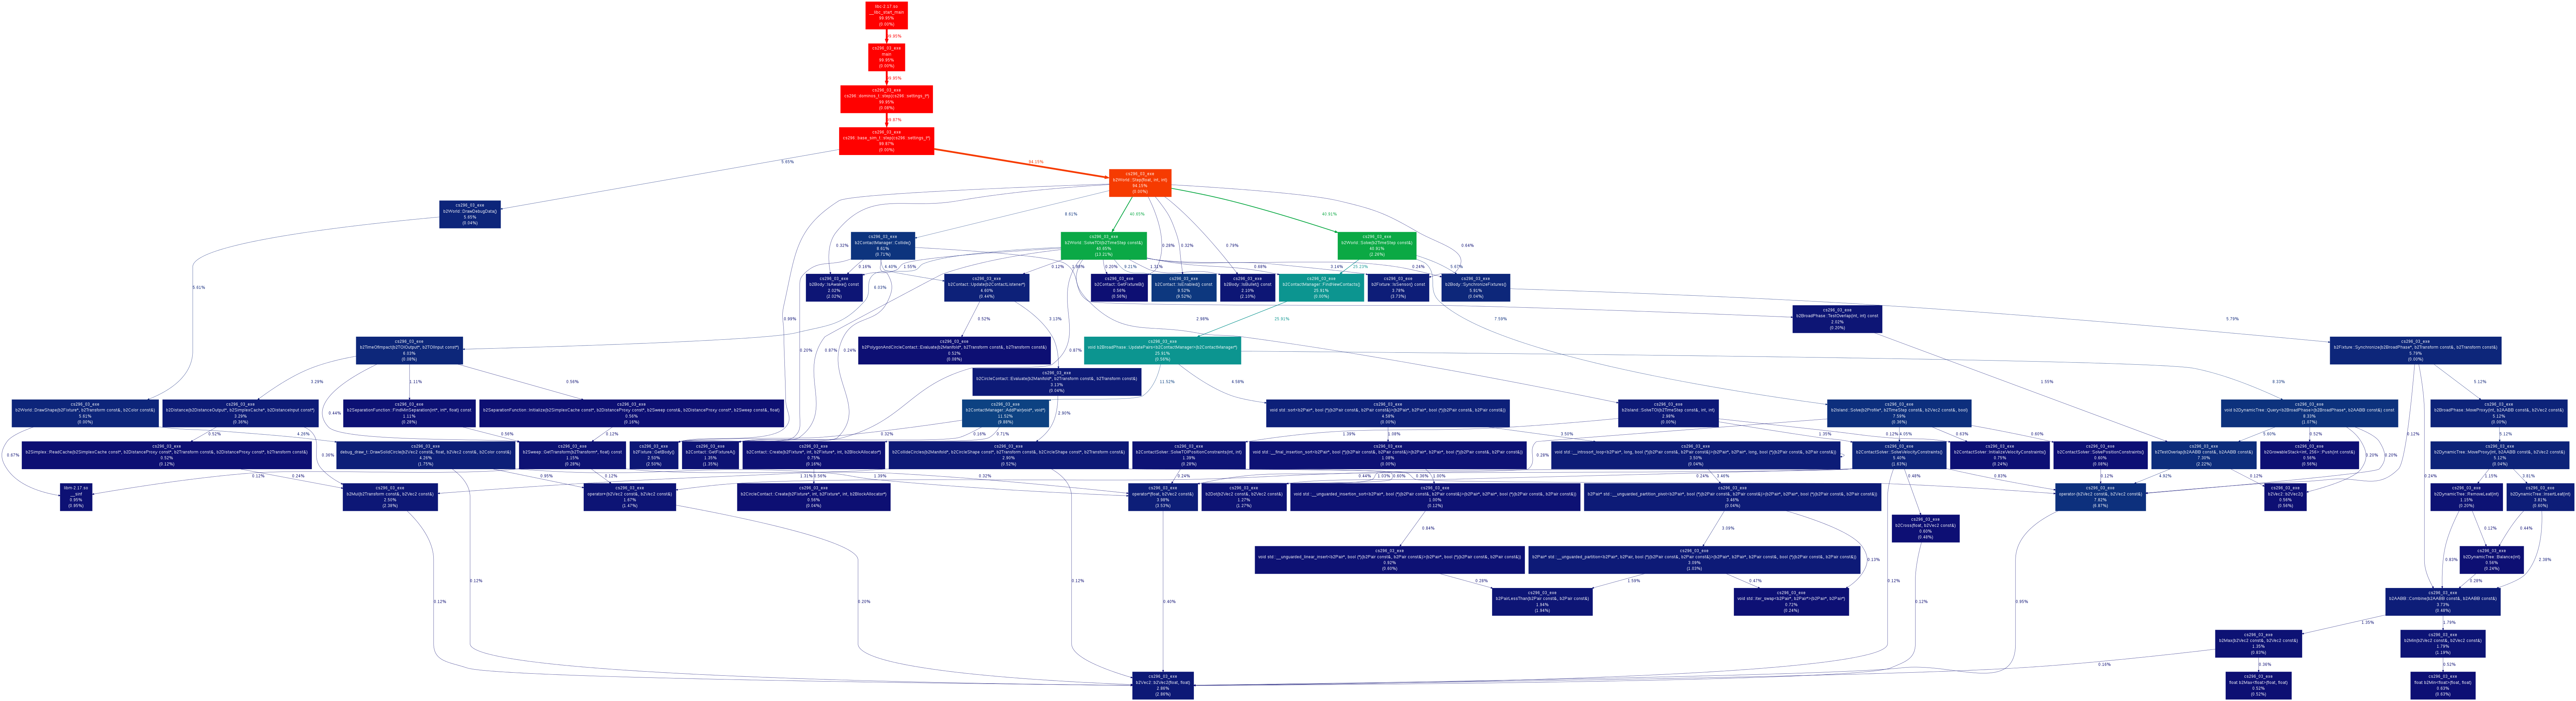
\includegraphics[width=\textwidth,height=\textheight,keepaspectratio]{output_d.png}
  \textbf{Callgraph for Debug Profile}
\end{center}
The debug profile is generated for suggestions concerned with debugging.
The debug profile generated by perf is quite well explained and contains a lot of calls.The profile shows that most of the time about 99 \% is consumed in the \texttt{base\_sim\_t} class and dominoes class.Out of this about 6 \% is consumed in Debug draw and  about ninety "\%" is consumed in the World generation which is also mainly concerned with functions like b2World solve, functions of b2 World Contact Manager,b2 World contact  solving for positions ,velocities and other parameters and b2 Fixtures as there are too many fixtures in the simulation.   
\subsubsection{Release}

\begin{center}
  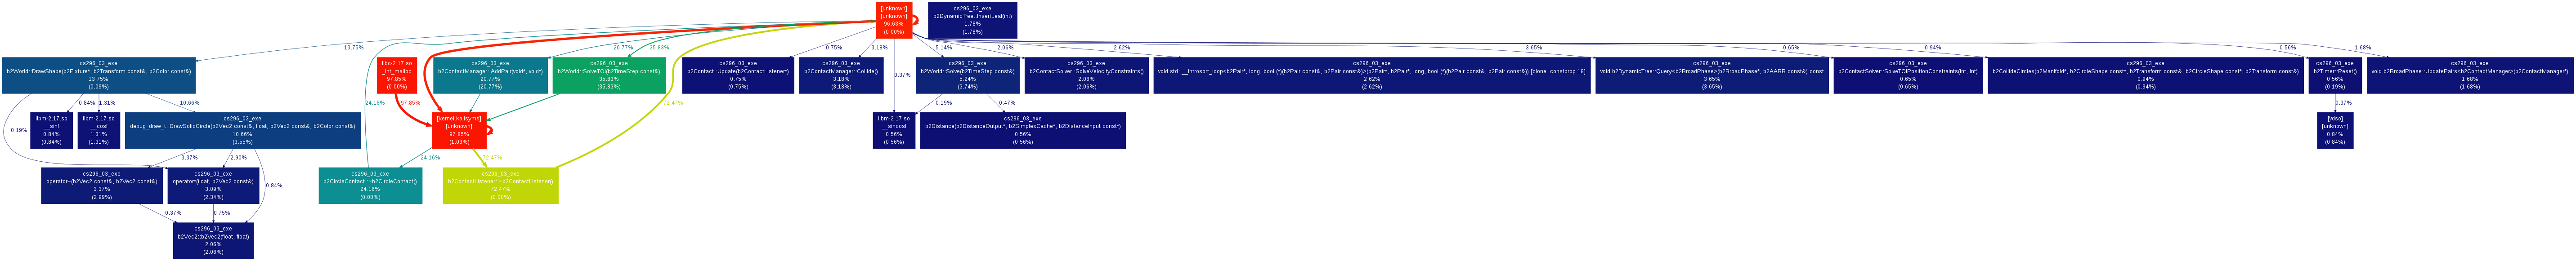
\includegraphics[width=\textwidth,height=\textheight,keepaspectratio]{output_r.png}
  \textbf{Callgraph for Release Profile}
\end{center}
The release profile uses the -On tags which help in internal optimizing.
The release profile generated by perf has relatively less calls.In this graph most of the time is used in call to the b2World:solve,b2ContactManager:add pairs,Draw shape function which inturn calls to DebugDraw functions.It has calls to solveVelocityConstraints and such functions but the percentage time is relatively less.The time within this  is also heavily consumed by the operators.
\subsection{Optimization}
The parts of the programs to be optimized are the ones  are the ones which consume more percentage of time(Some of them have been listed in descriptions like +,*,- operators and functions like b2Contactsolver and b2 Vec2 and b2World) and which debug does but release optimizes. \\
We could also try to optimize those functions which took time in both release and debug profile and the -On tag wasn't able to optimize them
like b2Dominoes and b2Fixtures.
\nocite{halliday}
\nocite{man}
\nocite{iforce2d}
\nocite{stackexchange}
\bibliography{g03_report}
\end{document}
